\section{Painting detection}
\label{sec:painting-detection}

The core of this work is the detection of paintings. For this purpose, an unsupervised segmentation algorithm was designed to extract all visible paintings in any arbitrary image. The essence of the algorithm is to associate straight lines that represent the enclosed region of a painting frame. For convenience, the detector is designed to find rectangular shapes when viewed head-on or quadrilateral shapes when viewed at a different angle.

\subsection{Proposed algorithm}
\label{subsec:proposed-algorithm}

The first step in the detection pipeline is to construct an edge map of a given single-channel image using the Canny operator. Since edge detection algorithms are heavily impacted by noise, the first step should always be to reduce the effects of noise by applying a filter. The original paper by John Canny \cite{Canny1986} suggested using a Wiener filter for optimally estimating the noise component of an image-noise two-component signal. Since this requires knowledge of the noise spectrum it is much easier to apply a Gaussian smoothing filter. All incoming images are resized to a width of 500 pixels and filtered using a 9x9 Gaussian kernel with $\sigma = 1$. The image size is fixed to ensure consistent results throughout the dataset and to speed up the calculations.  Images with higher resolution may cause suboptimal results of the smoothing kernel and would require a variable size of the kernel. The high and low threshold parameters of the Canny operator are calculated using the Otsu method \cite{Fang2009} \cite{greensted}. Its basic principle is to assign every pixel of the image to either foreground or background bucket and to calculate an optimal threshold value based on the intra-class variance. The resulting threshold value minimizes the sum of foreground and background spreads. The resulting edge map of figure \ref{fig:image-example} is shown in figure \ref{fig:edgemap-example}. Note that after applying the Canny operator, some detected edges are disconnected. The results can be improved by dilating the edge map using a 3x3 kernel.

\begin{figure}[htbp]
    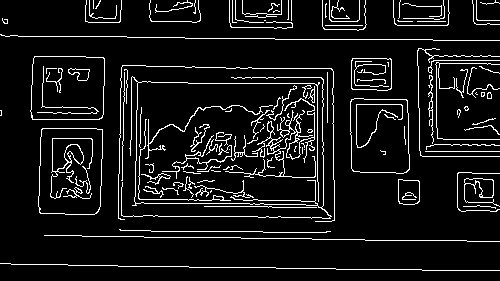
\includegraphics[width=\linewidth]{images/edgemap-example.png}
    \caption{Edgemap of figure \ref{fig:image-example}}
    \label{fig:edgemap-example}
\end{figure}

\textbf{Cv2.findContours} extracts contours using the binary edge map from the previous step. A contour is defined as a curve joining all the continuous points (along the boundary), having the same color or intensity \cite{opencvContours}. Thus the result of this function is a list of groups. Each group consists of points (that are connected to each other) in the binary image. To exclude contours that lie fully within other contours the retrieval mode can be set to \textbf{cv2.RETR\_EXTERNAL}. Contours are sorted by area and limited to the 25 largest to prevent small detected patches that are unusable by the matching algorithm anyway. The next step tries to select contours that are closely related to the shape of a painting frame (squares, rectangles, quadrilaterals, etc.). This implies that we first need to simplify each group of points to a general geometric shape so the corners can be assigned. First of all, the convex hull of the contour is generated and simplified using the \textbf{cv2.approxPolyDP} function to correct small errors in straight lines. Afterward, every contour may be considered a candidate painting if the simplified convex hull can be represented using four points (the corners of the quadrilateral) and its solidity is greater than 60\% (see equation \ref{eq:solidity}). The solidity check prevents the acceptance of contours that are an extreme mismatch compared to their respective convex hull.

\begin{equation}
    \label{eq:solidity}
    Solidity = \frac{Contour \; Area}{Convex \; Hull \; Area}
\end{equation}

The final step in the algorithm is to rectify every contour that satisfies the previous criteria. This is easily done as the corners of the quadrilaterals are known. The matching algorithm and subsequent steps require the inputs to be rectangular to ensure optimal results.

The rectified image crops are passed through the blur detection scheme from section \ref{subsec:blur-detection}. Blurry or vague crops are far more likely to cause a miss classification in the matcher. This mainly occurs when paintings are detected with an acute viewing angle.

\begin{figure}[htbp]
    \subfigure[All contours found on figure \ref{fig:image-example}]
    {
        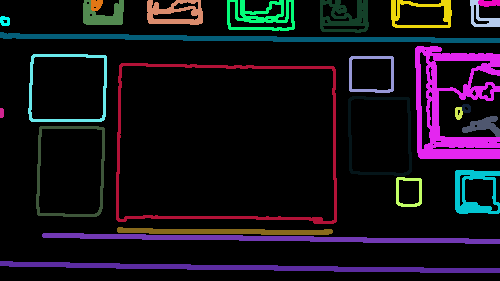
\includegraphics[width=.9\linewidth]{images/contours_all_example.png}
        \label{fig:contours_all}
    }
    \subfigure[Filtered contours, amount of corners and solidity checks applied]
    {
        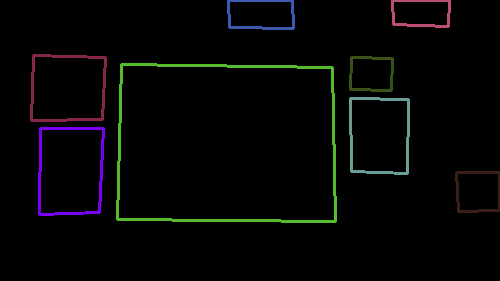
\includegraphics[width=.9\linewidth]{images/contours_filtered_example.png}
        \label{fig:contours_filtered}
    }
    \subfigure[Contours drawn on the original image]
    {
        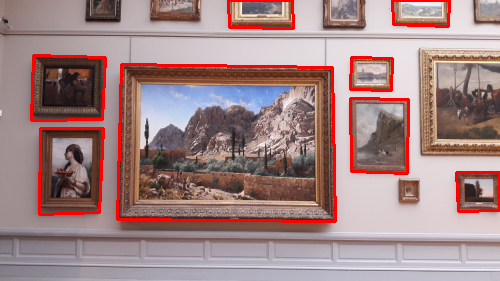
\includegraphics[width=.9\linewidth]{images/contours_filtered_image_example.png}
        \label{fig:contours_on_image}
    }
    \caption{Visualization of the contour filtering procedure (every color represents a different contour)}
    \label{fig:contours}
\end{figure}

\clearpage
\begin{strip}
    \centering
    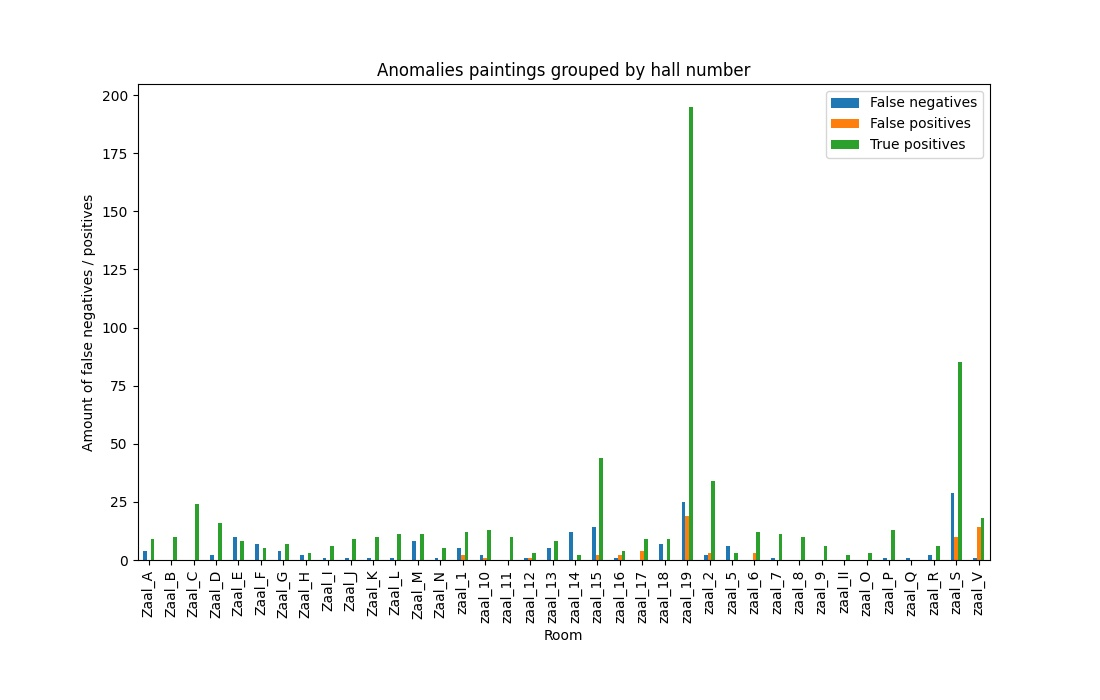
\includegraphics[width=\linewidth]{images/grouped_by_hall_include_TP.jpg}
    \captionof{figure}{Benchmark results displaying a histogram of true positives, true negatives and false negatives}
    \label{fig:benchmark-all}
\end{strip}

\begin{strip}
    \centering
    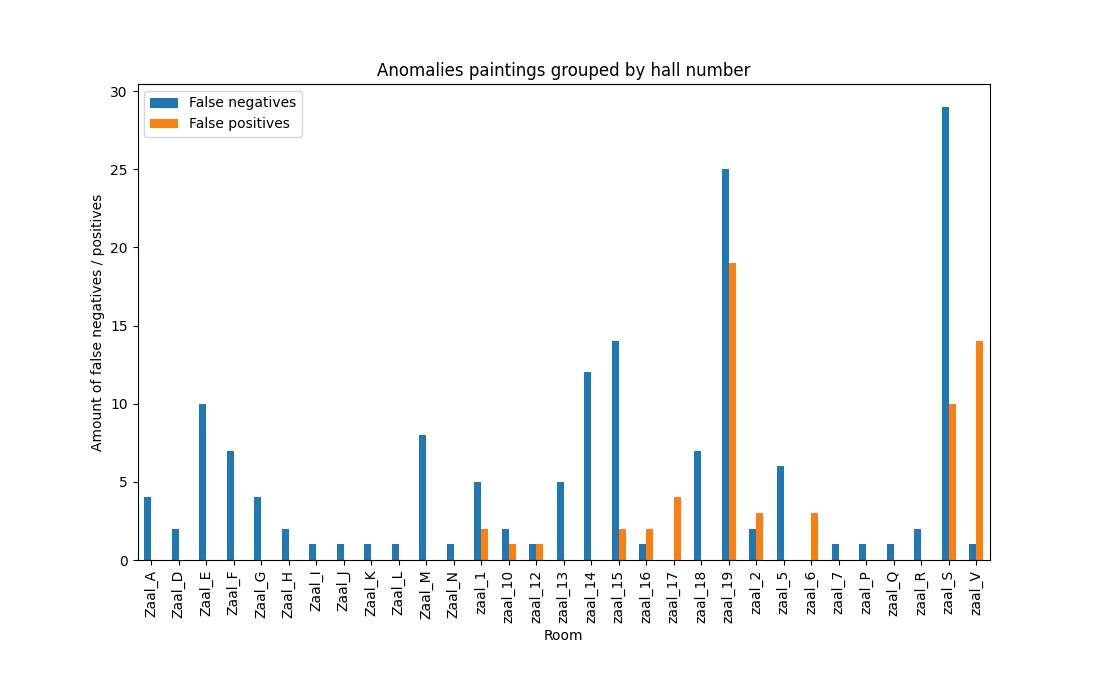
\includegraphics[width=\linewidth]{images/grouped_by_hall.jpg}
    \captionof{figure}{Benchmark results with true Positives omitted}
    \label{fig:benchmark-notp}
   
\end{strip}

\subsection{Benchmark results}

The quality of the painting detector was assessed using a validation dataset and a CSV file that contains the corners of all paintings in the images in the validation set. The results are shown as a confusion matrix in table \ref{tab:confusion_matrix_benchmark} and correspond to a $recall = 0.8065$, $precision = 0.9137$ and  $F1 = 0.8568$. For the detected paintings (646 detected paintings for 801 paintings in the dataset), we achieved an average intersection over union score (IOU) of $0.8934$. The distribution of IOU scores is displayed in figure \ref{fig:IOU-distribution} and is further elaborated on in section \ref{subsec:detection-failure}.

\begin{table}[htbp]
    \caption{Confusion matrix of the benchmark dataset}
    \begin{center}
        \begin{tabular}{l|l|c|c|c}
            \multicolumn{2}{c}{}&\multicolumn{2}{c}{Ground truth}&\\
            \cline{3-4}
            \multicolumn{2}{c|}{}&Positive&Negative&\multicolumn{1}{c}{Total}\\
            \cline{2-4}
            \multirow{2}{*}{Predicted}& Positive & $646$ & $61$ & $707$\\
            \cline{2-4}
            & Negative & $155$ &  & \\
            \cline{2-4}
            \multicolumn{1}{c}{} & \multicolumn{1}{c}{Total} & \multicolumn{1}{c}{$801$} & \multicolumn{    1}{c}{} & \multicolumn{1}{c}{$801$}\\
        \end{tabular}
    \end{center}
    \label{tab:confusion_matrix_benchmark}
\end{table}


\begin{figure}[htbp]
    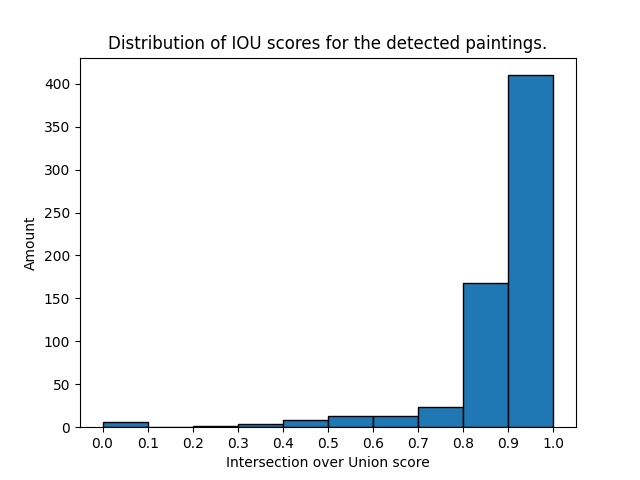
\includegraphics[width=\linewidth]{images/IOU_distribution.jpg}
    \caption{Intersection over union distribution of the detected paintings in the benchmark set}
    \label{fig:IOU-distribution}
\end{figure}



\subsection{Common causes of failure}
\label{subsec:detection-failure}

Figure \ref{fig:common-error-noframe} shows one of the most common detection errors, the exclusion of the painting frame. These are detections that correspond with an IOU score between $0.75$ and $0.95$ (see figure \ref{fig:IOU-distribution}). This doesn't pose too much of a problem since the actual painting information is preserved. However, all the frame information which may contain strong keypoints to match is lost. Those keypoints may be included in the database representation of the ground truth images.

Other common circumstances when a painting is not or less accurately detected are:

\begin{enumerate}
    \item Painting frame is not completely visible in the image.
    \item The difference between the painting background and the wall is not strong enough to be detected as a line.
    \item Shadows caused by the painting frame commonly form a strong edge and are included in the painting contour. This causes a lower IOU score for the detection.
    \item Next to most of the paintings hangs a small plaque (containing information) that is falsely classified as a painting when its color is different from the wall color.
    \item Hall 14 is plastered with a wallpaper that contains quadrilateral shapes which interfere with the contours of the paintings and causes a very large amount of false negatives. This behavior can be verified using figure \ref{fig:benchmark-notp}.
\end{enumerate}

\begin{figure}[htbp]
    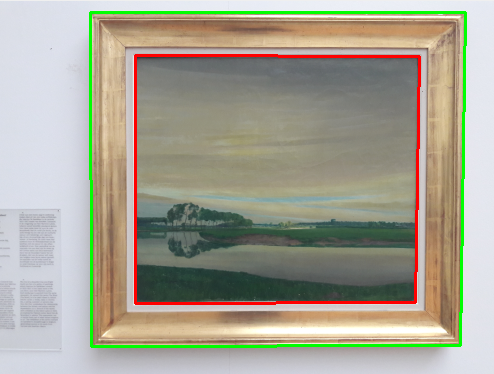
\includegraphics[width=\linewidth]{images/common-error-noframe.png}
    \caption{One of the most common errors (the picture frame is not included in the detection), green shows the ground truth bounding box and red is the predicted one}
    \label{fig:common-error-noframe}
\end{figure}